\chapter{Design Sensitivity Analysis}
In this chapter, the concept behind discrete and continuum sensitivity formulation is discussed and the general approach for deriving the sensitivity equations is presented. The two sensitivity analysis techniques are applied to a heat transfer benchmark problem where the sensitivity of response to the shape of the domain is calculated. This problem is also used in the next chapter for implementation of different immersed boundary methods. The difference between local and total formulation of the sensitivity response is discussed and finally the independence of continuum sensitivity formulation to discretization method is proven. This enables use to reuse the solver of governing equation to calculate the sensitivity response. This is typically not possible for discrete sensitivity formulation.

% ======================================================================================
\section{General formulation}
The general computational domain is defined as shown in Figure \ref{fig:C2_continuumDomain}. The response variable on this domain can be from the fluid, i.e. pressure or velocity, or the solid, i.e. displacements. Nevertheless, the response is calculated using a governing equation subject to boundary conditions. In this work, the governing equation and boundary conditions are represented in the functional form as shown in Equation \eqref{eq:C2_governingEquationAndBC}.

\begin{subequations}
\begin{gather}
	\mathbf{A}(\mathbf{u}, t; \mathbf{b}) = \mathbf{f}(\mathbf{x}, t; \mathbf{b})
	\quad \text{on} \quad \Omega
	\\
	\mathbf{B}(\mathbf{u}, t; \mathbf{b}) = \mathbf{g}(\mathbf{x}, t; \mathbf{b})	
	\quad \text{on} \quad \Gamma
\end{gather}\label{eq:C2_governingEquationAndBC}
\end{subequations}

where $\mathbf{A}$ is the governing equation such as Navier-Stokes equations or elastic equations and $\mathbf{B}$ is the boundary condition definition. $\mathbf{u}$ is the response variable such as displacement or pressure. $t$ is time, $\mathbf{b}$ is the design variable such as shape or size, and $\mathbf{x}$ is the spatial coordinate. $\mathbf{f}$ and $\mathbf{g}$ is the value of governing equation and boundary condition. The sensitivity of response variable with respect to $i$-th design variable $b_i$, $\partial \mathbf{u}/\partial b_i$, can be calculate using some sensitivity analysis technique. This is done in the following sections.

The total sensitivity of response variable, $\mathbf{u}$ with respect to the $i$-th design variable is written as

\begin{equation}\label{eq:C2_totalSensitivityDef}
	\frac{D \mathbf{u}}{D b_i} = 
	\frac{\partial \mathbf{u}}{\partial b_i} + 
	\frac{\partial \mathbf{u}}{\partial \mathbf{x}} \cdot
	\frac{\partial \mathbf{x}}{\partial b_i} 
\end{equation}

The total derivative is known as material derivative in continuum mechanics \cite{mase2009continuum}. This total sensitivity defines the change of response variable, $\mathbf{u}$, subjected to design variable and space dependent changes. The material derivative consists of the local derivative, $\partial \mathbf{u}/\partial b_i$, plus the convective term, $\partial \mathbf{u}/\partial \mathbf{x} \cdot \partial \mathbf{x}/\partial b_i$. The local derivative is the measure of change in the response variable due to change in the design parameter. Whereas, the convective term accounts for the movement of this point in space due to change in the design variable. This is specially applicable to shape sensitivity calculating where the change in design variable, will cause the material points to move \cite{cross2014local}. The convective term consists of two separate gradients: i) $\partial \mathbf{u} / \partial \mathbf{x}$ which represents the spatial gradient of the response variable in the domain, and ii) $\partial \mathbf{x} / \partial b_i$ which defines the sensitivity of the spatial domain with respect to the change in design variable. The later defines how the computational nodes moves as the design variable changes. The response variable spatial gradient term can be calculated using the analysis results, using finite difference approach or derivative of shape functions in FEA formulation. Calculation of domain sensitivity, $\partial \mathbf{x} / \partial b_i$, requires more attention.

A common approach to calculate the domain sensitivity, is to use the same techniques used to deform the body-conformal mesh in a CFD simulation. These methods are usually based on representing the computational grid as a system of springs that connected to each other at the nodes. This system can be modeled and solved using structural analysis techniques, where the sensitivities can be easily added to its formulation. This is effectively a shape sensitivity analysis for the structural analyses \cite{haftka1986structural}. This step can be removed from the analysis if the computational domain does not affected by design variable since $\partial x/\partial b$ is equal to zero for this case. This is removes the extra step of doing the structural shape sensitivity analysis for the mesh and also response variable gradient calculation. As mentioned in Chapter \ref{ch:introduction}, by using the immersed boundary method the mesh definition is decoupled from the boundary shape. Therefore, domain sensitivity is equal to zero \cite{gobal2014continuum}. This is one of the reasons to use the immersed boundary calculation since it reduces the cost of the simulation. This is discussed in more details in Chapter \ref{ch:immersedBoundary}.

% ======================================================================================
\section{Benchmark case}
To compare the discrete and continuum sensitivity analysis we chose the one-dimensional heat transfer analysis in a rod. The temperature in governing by the Laplace equation as shown in Equation \eqref{eq:C2_laplaceEquation}.

\begin{equation}\label{eq:C2_laplaceEquation}
	\frac{\partial^2 T}{\partial x^2} = 0
\end{equation}

where $T$ is the temperature and $x$ is spatial variable. The boundary conditions are defined as constant temperatures at the two ends of the domain as shown in Figure \ref{fig:C2_benchmarkCase}. The length of domain is selected as $L$.

\begin{figure}[h]
	\centering
	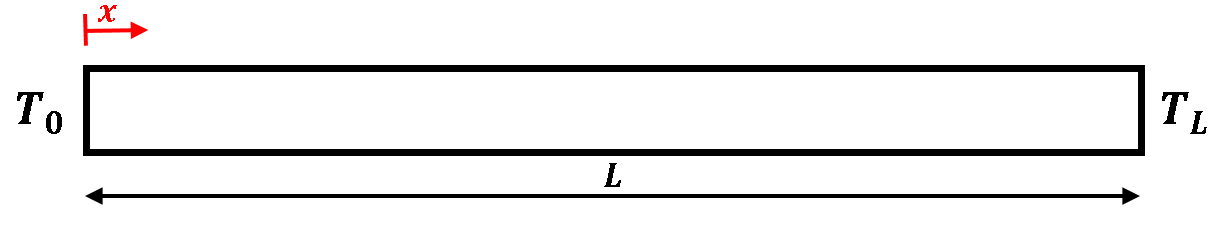
\includegraphics[width=14.00cm]{Chapter_2/figure/benchmark_case.png}
	\caption{One dimensional domain with heat conduction.}
	\label{fig:C2_benchmarkCase}
\end{figure}

The analytical solution of Equation \eqref{eq:C2_laplaceEquation} can be written as follows

\begin{equation}\label{eq:C2_benchmarkCaseAnalyticalSolution}
	T = \frac{T_L - T_0}{L} x + T_0
\end{equation}

The analytical sensitivity of the temperature with respect to beam's length can be calculated by differentiating Equation \eqref{eq:C2_benchmarkCaseAnalyticalSolution} with respect to $L$.

\begin{equation}
	\frac{\partial T}{\partial L} = -\frac{T_L - T_0}{L^2} x
\end{equation}

Since the analytical derivatives are known, we can compare it to the discrete and continuous sensitivity results.

% ======================================================================================
\section{Discrete sensitivity formulation}
To formulate the discrete sensitivity equation, we start by discretizing the governing equation \eqref{eq:C2_laplaceEquation} using finite difference method. It should be noted that the finite difference is used for discretization of continuum governing equation and not sensitivity calculation. The design variable effects the shape of the domain which is the distance between the nodes in the discrete manner. Therefore, for the sake of sensitivity analysis it is required to keep the nodal distances in the discretized solution as well. We use 6 nodes to discretize the domain as shown in Figure \ref{fig:C2_discretizedDomain}.

\begin{figure}[h]
	\centering
	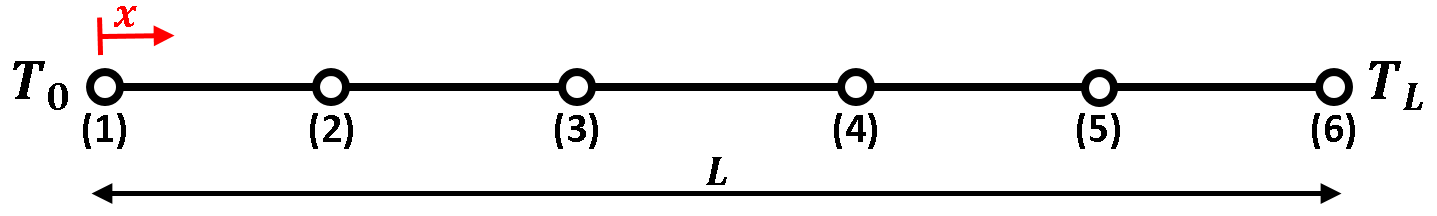
\includegraphics[width=14.00cm]{Chapter_2/figure/benchmark_case_computational_domain.png}
	\caption{One dimensional computational domain for heat conduction.}
	\label{fig:C2_discretizedDomain}
\end{figure}

To discretize Equation \eqref{eq:C2_laplaceEquation}, the first step is to approximate the second derivative. This is done by writing the Taylor series expansion at at arbitrary location $x_i$.

\begin{equation*}
	T(x) = 
	T(x_0) + 
	\frac{\partial T}{\partial x} \bigg|_{x_i} (x - x_i) + 
	\frac{\partial^2 T}{\partial x^2} \bigg|_{x_i} (x - x_i)^2 + 
	\mathcal{H} . \mathcal{O} . \mathcal{T}
\end{equation*}

To approximate the second derivative at the arbitrary node $x_i$ using central method we need to use the neighbouring nodes. The second order approximation for the second order derivative of central difference method is shown in Equation \eqref{eq:C2_finiteDifferenceSchemes}. The discretized equations are differentiated with respect to shape design variable. This requires the nodal distances to be included in the discretized equations. To maintain the generality, we assume that distance of node $T_i$ to $T_{i+1}$ is $\Delta_i$ and the distance of node $T_i$ to $T_{i-1}$ is $\Delta_{i-1}$.

\begin{equation}\label{eq:C2_finiteDifferenceSchemes}
	\frac{\partial^2 T}{\partial x^2} = 
	\frac{T_{i-1} \Delta_{iL} - 
	      T_{i} (\Delta_{iL} + \Delta_{iR}) + 
	      T_{i+1} \Delta_{iR}}
	     {\dfrac{1}{2} \left[ \Delta_{iL} \Delta_{iR}^2 + 
	                         \Delta_{iL}^2 \Delta_{iR} \right]}
\end{equation}

The approximation of the second derivative in Equation \eqref{eq:C2_laplaceEquation} is done using definitions in Equation \eqref{eq:C2_finiteDifferenceSchemes} for each node excluding the boundary nodes. As mentioned in the previous section, the nodal values at boundary nodes, $(1)$ and $(2)$ are known. The discretized governing equations is written in the matrix form as shown in Equation \eqref{eq:C2_laplaceEquationMatrixForm}.

\begin{equation}\label{eq:C2_laplaceEquationMatrixForm}
	\begin{bmatrix}
		\frac{-2}{\Delta_{1} \Delta_{2}} &
		\frac{2}{\Delta_{1} \Delta_{2} + \Delta_{1}^2} &
		0 &
		0 &
		\\
		\frac{2}{\Delta_{3}^2 + \Delta_{2} \Delta_{3}} & 
		\frac{-2}{\Delta_{2} \Delta_{3}} &
		\frac{2}{\Delta_{2} \Delta_{3} + \Delta_{2}^2} &
		0
		\\
		0 &
		\frac{2}{\Delta_{4}^2 + \Delta_{3} \Delta_{4}} & 
		\frac{-2}{\Delta_{3} \Delta_{4}} &
		\frac{2}{\Delta_{3} \Delta_{4} + \Delta_{3}^2} &
		\\
		0 &
		0 &
		\frac{2}{\Delta_{5}^2 + \Delta_{4} \Delta_{5}} & 
		\frac{-2}{\Delta_{4} \Delta_{5}}
	\end{bmatrix}
	\begin{bmatrix}
		T_2 \\
		T_3 \\
		T_4 \\
		T_5
	\end{bmatrix}
	=
	-\begin{bmatrix}
	 	\frac{2T_1}{\Delta_{2}^2 + \Delta_{1} \Delta_{2}} \\
 		0 \\
		0 \\
		\frac{2T_6}{\Delta_{5} \Delta_{4} + \Delta_{5}^2}
	\end{bmatrix}
\end{equation}

To verify the discretization process, we compare the analytical solution of this problem with the result of Equation \eqref{eq:C2_laplaceEquationMatrixForm} in Figure \ref{fig:C2_verificationOfSolver}. For this problem we choose $T_1 = 0$, $T_6 = 1$, and $L = 1$.  As shown in this figure, the discrete and continuum results match very well.

\begin{figure}[h]
	\centering
	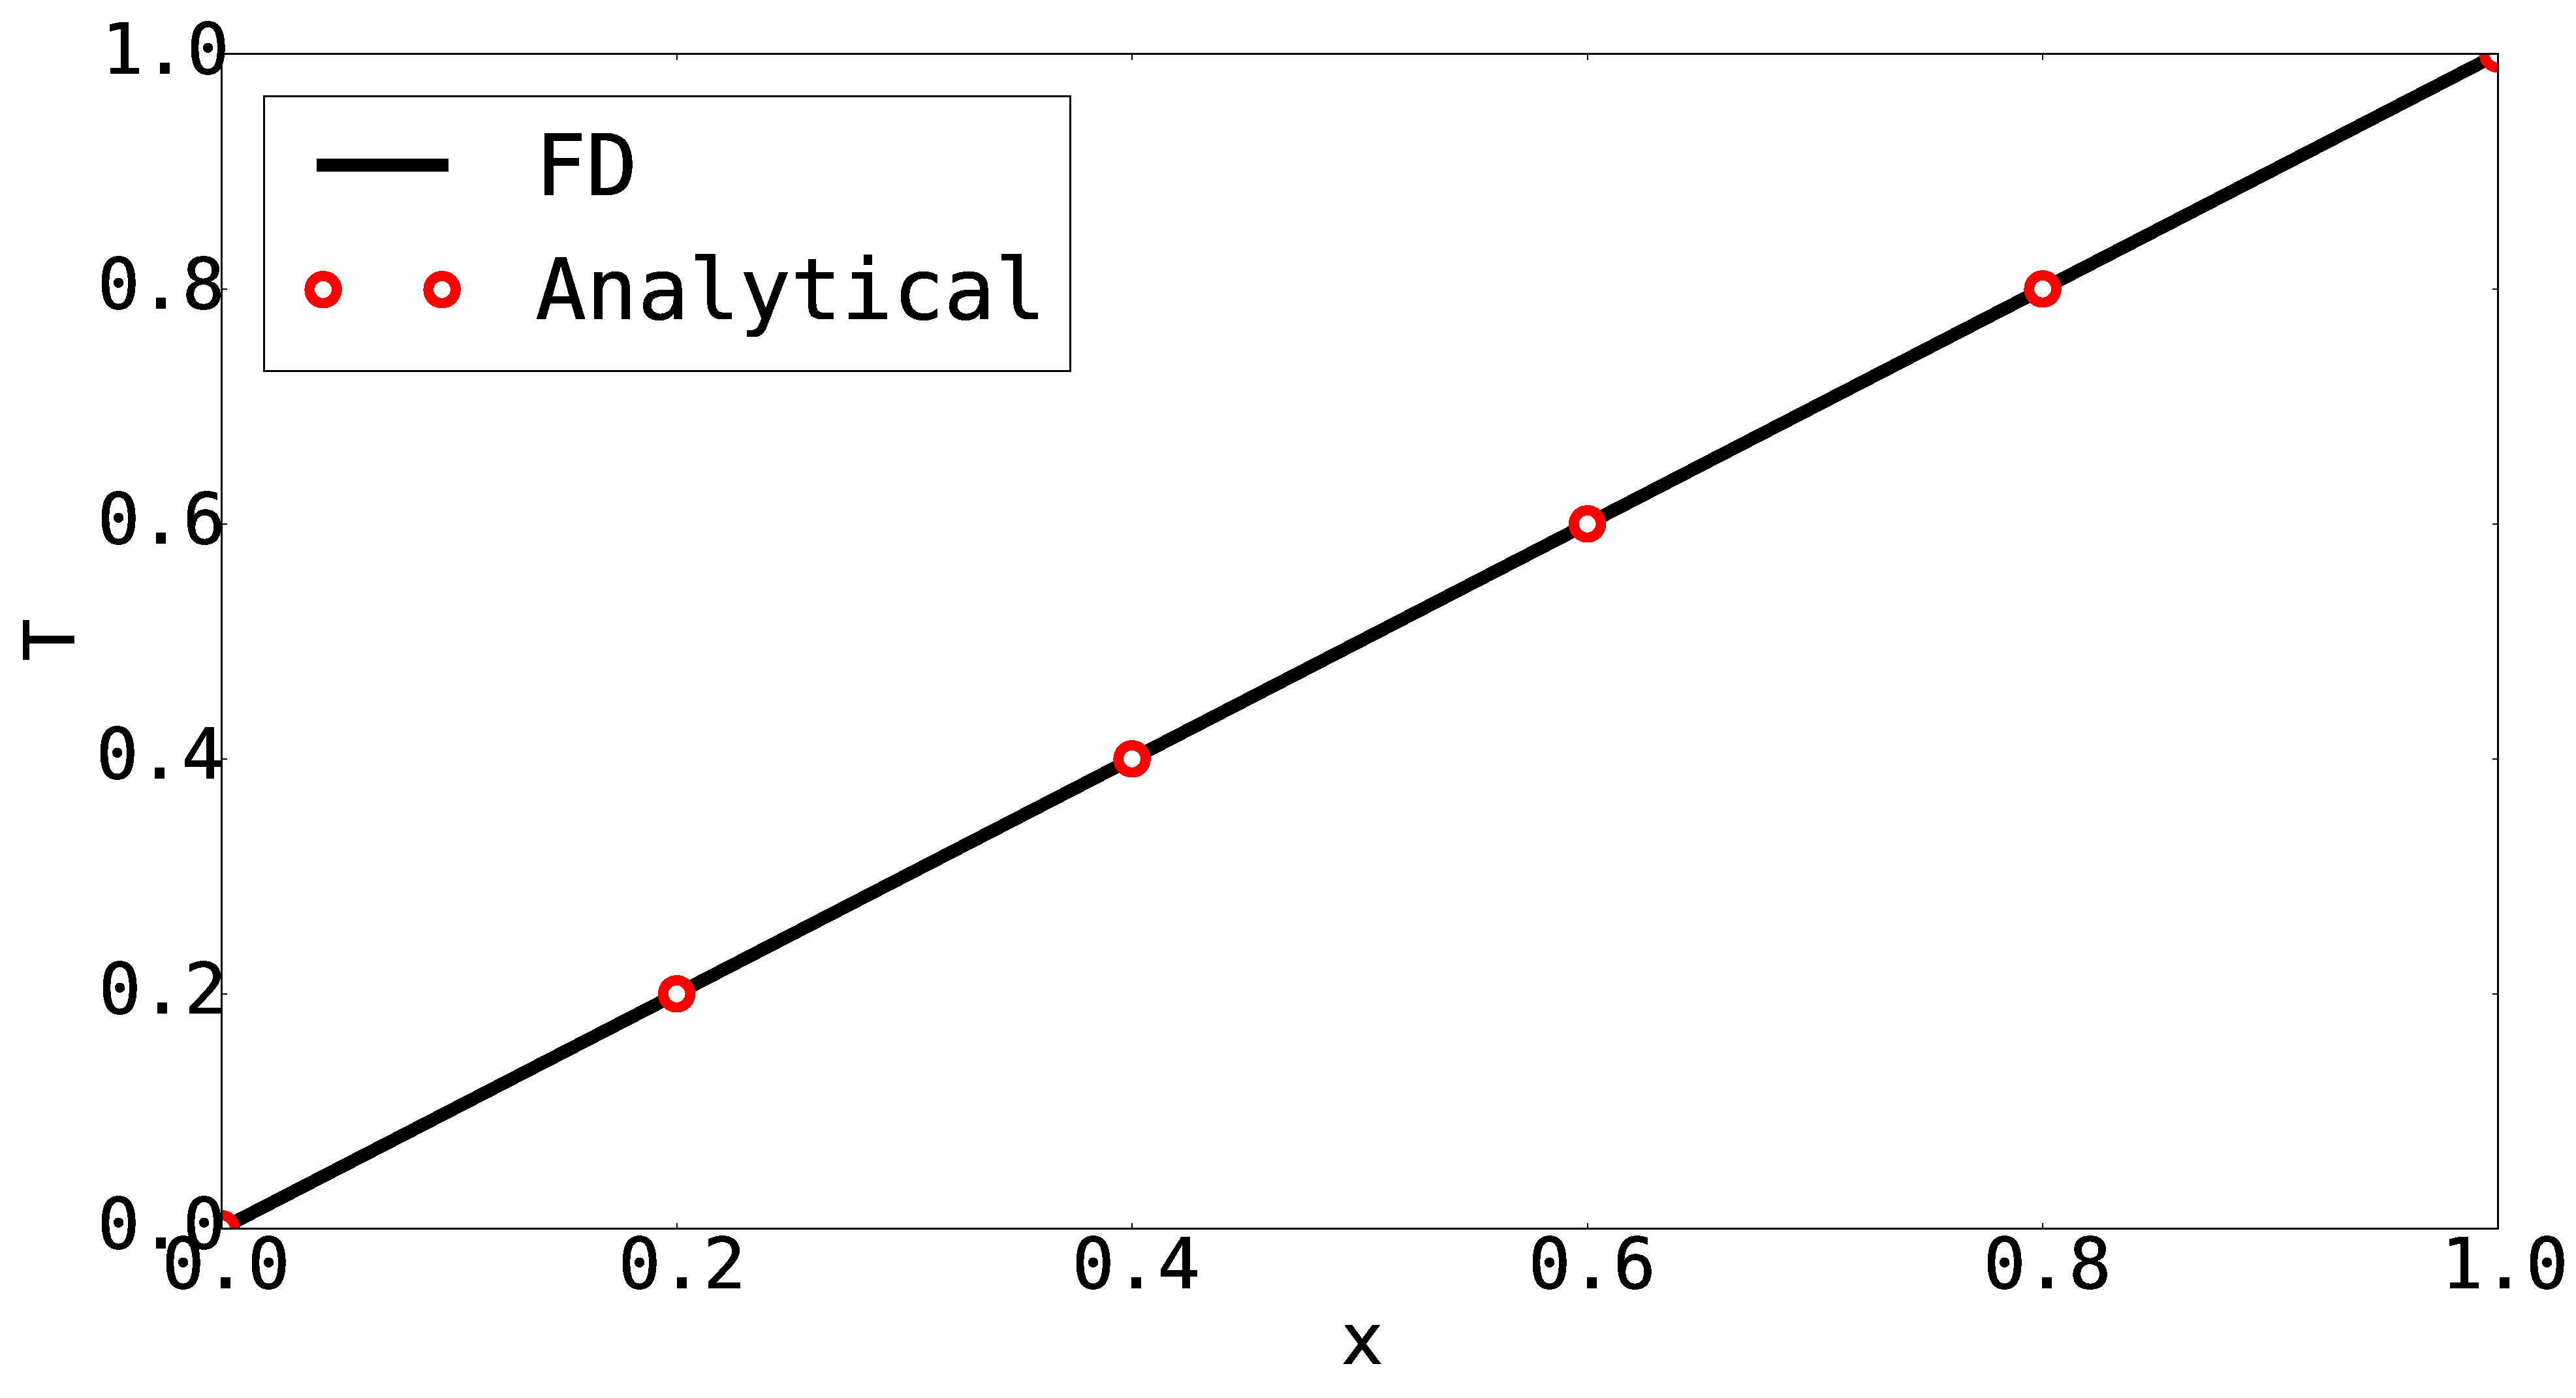
\includegraphics[height=9.00cm]{Chapter_2/figure/finitedifference_vs_analytical.eps}
	\caption{Comparison between the analytical and finite difference solution for 1D heat equation.}
	\label{fig:C2_verificationOfSolver}
\end{figure}

The sensitivity equations are derived by differentiating the discretized governing equation of \eqref{eq:C2_laplaceEquationMatrixForm} with respect to the length of the domain. We assume that the change in the length, only affects the nodal distance between the last two nodes and the rest remain unchanged. This means that only the node next to the boundary will move and the rest of nodes will be stationary. This is required to make sure that the sensitivity at each of the degrees of freedom is only a function of change in shape not movement of material nodes.

To calculate the sensitivities, It is required to calculate the derivative of nodal distances in Equation \eqref{eq:C2_laplaceEquationMatrixForm} with respect to $L$. For a equally space grid, the nodal distance is written as

\begin{equation*}
	\Delta x = \frac{L}{n - 1}
\end{equation*}

where $L$ is the length of the domain, and $n$ is the number of nodes chosen to discretize the domain. The sensitivity of nodal distances to the length of the domain is calculated as

\begin{equation}\label{eq:C2_nodeDistanceSensitivity}
	\frac{\partial \Delta x}{\partial L} = \frac{1}{n-1}
\end{equation}

The discretized equation is differentiated as shown in Equation \eqref{eq:C2_laplaceEquationMatrixFormSensitivity}. It should be noted that since only the adjacent node to the boundary is affected by shape change, only that element in the matrix derivative has a value.

\begin{equation}\label{eq:C2_laplaceEquationMatrixFormSensitivity}
	\begin{bmatrix}
		-2 & 1 & 0 & 0 \\
		1 & -2 & 1 & 0 \\
		0 & 1 & -2 & 1 \\
		0 & 0 & 1 & -2
	\end{bmatrix}
	\begin{bmatrix}
		T'_2 \\
		T'_3 \\
		T'_4 \\
		T'_5
	\end{bmatrix}
	=
	\frac{1}{2} \frac{\partial \Delta}{\partial L} \frac{1}{\Delta}
	\begin{bmatrix}
		0 \\
		0 \\
		0 \\
		T_6
	\end{bmatrix}
	-
	\underbrace{
	\frac{1}{2} \frac{\partial \Delta}{\partial L} \frac{1}{\Delta}
	\begin{bmatrix}
		0 & 0 & 0 & 0 \\
		0 & 0 & 0 & 0 \\
		0 & 0 & 0 & 0 \\
		0 & 0 & -3 & 1
	\end{bmatrix}
	\begin{bmatrix}
		T_2 \\
		T_3 \\
		T_4 \\
		T_5
	\end{bmatrix}}_\text{effect of shape change}
\end{equation}

In order to better study above we mention the general sensitivity equation in the discrete form. Assume the the continuum governing equation, can be written in the discrete form as

\begin{equation*}
	\left[ K \right] \left[ U \right] = \left[ F \right]
\end{equation*}

where $[K]$ is the discrete operator that represents the governing equation, $[U]$ is the vector of response variable defined at each of the degrees of freedom, and $[F]$ is the vector of the boundary conditions. The sensitivity of this system with respect to design variable $b$ is derived as

\begin{equation*}
	\left[ K \right] \left[ \frac{\partial U}{\partial b} \right] = 
	\left[ \frac{\partial F}{\partial b} \right] - 
		\left[ \frac{\partial K}{\partial b} \right] \left[ U \right]
\end{equation*}

By comparing above equation with Equation \eqref{eq:C2_laplaceEquationMatrixFormSensitivity}, we can see that the last term represents the change in the stiffness matrix. This depends on how the governing equations are discretized. Therefore, to do the sensitivity analysis it is required to know how this matrix is put together so it can be differentiated. This is not possible in most cases since the details of discretization is not known for the commertial software packages.

To verify the results of Equation \eqref{eq:C2_laplaceEquationMatrixFormSensitivity}, we compared it with the analytical sensitivity results are shown in Figure \ref{fig:C2_discreteSensitivityVerification}.

\begin{figure}
	\centering
	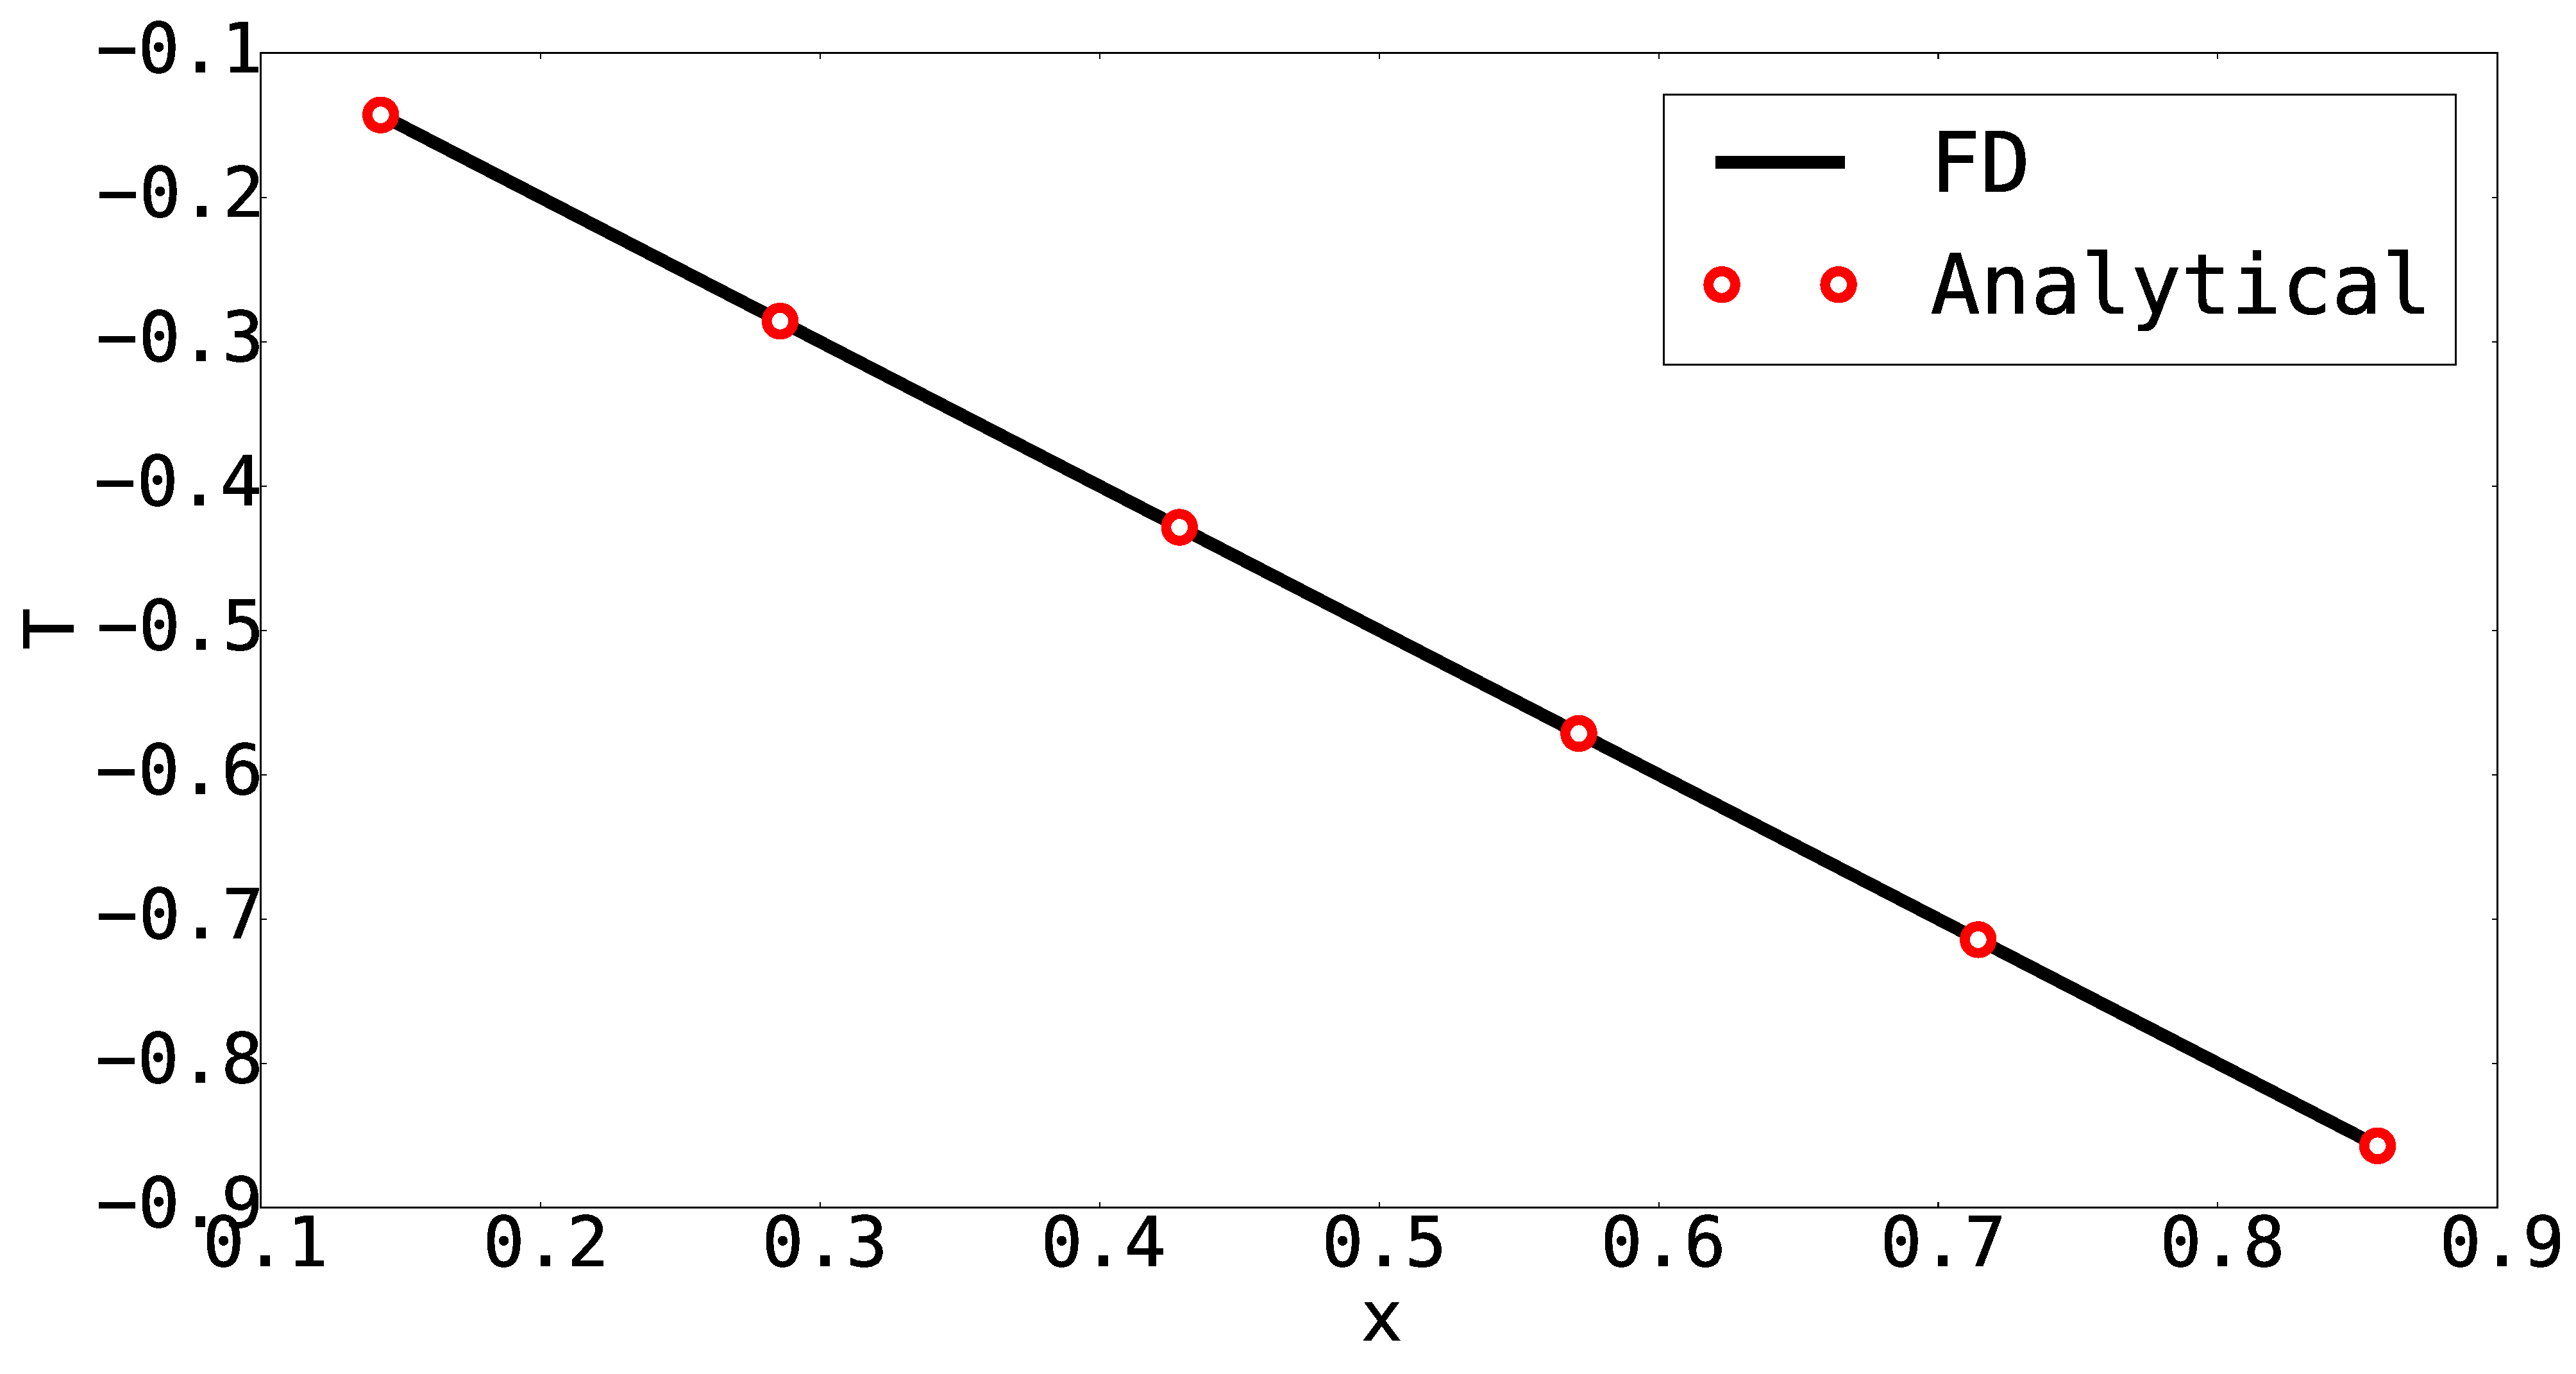
\includegraphics[height=9.00cm]{Chapter_2/figure/SA_finitedifference_vs_analytical.eps}
	\caption{Sensitivity analysis verification.}
	\label{fig:C2_discreteSensitivityVerification}
\end{figure}

% ======================================================================================
\section{Continuum sensitivity formulation}
For a continuum system, the governing equations and boundary conditions can be written as

\begin{subequations}\label{eq:C2_continuumGoverningEquation}
\begin{align}
	A(u, t; b) &= 0 \quad \text{on } \Omega \\
	B(u, t; b) &= g(x, t; b) \quad \text{on } \Gamma \\
\end{align}	
\end{subequations}

where $u$ is the response variable, i.e. displacement or pressure, $t$ is time, $x$ is the spatial coordinate, and $b$ is the design variable that can be used to control the solution. $A$ and $B$ are continuum functions that define the governing equations and boundary conditions respectively. It should be noted that the governing equation is written in the residual form where its value needs to be equal to zero when $u$ is the solution at time $t$. $g$ is the value of the boundary condition of the defined system. To calculate the sensitivity of response, it is required to calculate the total derivative of Equation \eqref{eq:C2_continuumGoverningEquation}. This is broken into calculating the local sensitivity of the system of governing equation followed by converting the local sensitivities to their total form using Equation \eqref{eq:C2_totalSensitivityDef}.

The governing equation of \eqref{eq:C2_continuumGoverningEquation} is differentiated as follows

\begin{subequations}\label{eq:C2_continuumSensitivityFormulation}
\begin{align}
	A(u', t; b) + A'(u, t; b) &= 0 \quad \text{on } \Omega \\
	B(\dot{u}, t; b) + \dot{B}(u, t; b) &= \dot{g}(x, t; b) \quad \text{on } \Gamma \\
\end{align}	
\end{subequations}

where $u'$ and $\dot{u}$ are local and total derivative which are defined as follows

\begin{subequations}
\begin{align*}
	(\text{ })' &= \frac{\partial (\text{ })}{\partial b} \\
	\dot{(\text{ })} &= \frac{D (\text{ })}{D b}
\end{align*}
\end{subequations}

It should be noted that the governing equations are differentiated in the local form and the boundary conditions are differentiated in the total form. Local differentiation of the governing equations enables us to treat the solver nonintrusively. However, in order to capture the effect of shape change, the boundary conditions need to be differentiated in total form. The boundary condition is further simplified by assuming linearly. This is a valid assumption for many practical cases such structural analysis or computational fluid dynamics. The boundary conditions are usually in the form of known gradient or value, i.e. outflow and free-slip wall for CFD and predefined displacement for structural analysis, at the boundary. It should be noted that this assumption is not valid for problems such as contacts. The boundary condition is written as

\begin{align}\label{eq:C2_linearSAboundaryCondtions}
\begin{split}
	B(\dot{u}, t; b) &= \dot{g}(x, t; b) \Rightarrow \\
	B(u', t; b) &= \dot{g}(x, t; b) - B(\frac{\partial u}{\partial x} \cdot \frac{\partial x}{\partial b}, t; b)
\end{split}
\end{align}

To study the differentiated governing equation of Equation \eqref{eq:C2_continuumSensitivityFormulation}, we will assume two situations: i) linear analysis, ii) nonlinear analysis.

For the linear analysis, the governing  of \eqref{eq:C2_continuumSensitivityFormulation} is written as

\begin{equation}\label{eq:C2_linearSAgoverningEquation}
	A(u', t; b) = 0 
\end{equation}

This is valid since for the linear case, the differential operators of the governing equation does not depend on the response variable, $u$. To explain this concept, we look at the transient heat conduction in 1D domain. The governing equations are defined as

\begin{equation}\label{eq:C2_transientHeatCondtionGE}
	\frac{\partial^2 T}{\partial x^2} = \frac{1}{\alpha} \frac{\partial T}{\partial t}
\end{equation}

where $T$ is the temperature, $x$ is spatial coordinate, $t$ is time, and $\alpha$ is is the thermal diffusivity ($k/\rho c_p$). This equation can be differentiated with respect to design variable $b$ as shown in the following equation.

\begin{equation*}
	\frac{\partial}{\partial b}
	\left( \frac{\partial^2 T}{\partial x^2}\right) = 
	\frac{\partial}{\partial b}
	\left( \frac{1}{\alpha} \frac{\partial T}{\partial t}\right)
\end{equation*}

Due to linearity of the differential operators we can change the order of differentiation as follows

\begin{equation}\label{eq:C2_transientHeatCondtionSA}
	\frac{\partial^2}{\partial x^2}
	\left( \frac{\partial T}{\partial b} \right) = 
	\frac{1}{\alpha} \frac{\partial}{\partial t}
	\left( \frac{\partial T}{\partial b}\right)
\end{equation}

By comparing Equations \eqref{eq:C2_transientHeatCondtionGE} and \eqref{eq:C2_transientHeatCondtionSA} we can see that the differential operators, $\partial^2 /\partial x^2$, and $\partial /\partial t$ remain unchanged. Therefore, same analysis can be used for solving this system of governing equations for the sensitivity variable, $\partial T/\partial b$.

For nonlinear problems, the differential operators are functions of response variable as well. For example, the incompressible Euler's equation for a 2D flow is derived as

\begin{subequations}\label{eq:C2_eulerEquations}
\begin{gather}
	\frac{\partial u}{\partial t} +
	u \frac{\partial u}{\partial x} + v \frac{\partial u}{\partial y} +
	\frac{\partial p}{\partial x} = 0 
	\\
	\frac{\partial v}{\partial t} +
	u \frac{\partial v}{\partial x} + v \frac{\partial v}{\partial y} +
	\frac{\partial p}{\partial y} = 0
\end{gather}
\end{subequations}

where $u$ and $v$ are the velocity components in $x$ and $y$ directions respectively. $p$ is the pressure, $t$ is time, $x$, and $y$ are spatial coordinates. We can rewrite Equation \eqref{eq:C2_eulerEquations} in terms of differential operators too.

\begin{subequations}
\begin{gather*}
	\mathcal{T} u +
	\mathcal{C} u +
	\mathcal{G}_x p = 0 
	\\
	\mathcal{T} v +
	\mathcal{C} v +
	\mathcal{G}_y p = 0 
\end{gather*}
\end{subequations}

where $\mathcal{T}$ is the time derivative operator ($\partial /\partial t$), $\mathcal{C}$, is the convective operator ($u \partial / \partial x + v \partial / \partial y$). $\mathcal{G}_x$ and $\mathcal{G}_y$ are gradient operators in $x$ and $y$ respectively ($\partial /\partial x$ and $\partial /\partial y$). The gradient and time derivative operators are linear, therefore they can be treated as shown in the previous paragraphs. On the other hand, the convective operator is nonlinear and it should be differentiated alongside response variables as well. As a result, the sensitivity equations can be written in the operator form as

\begin{subequations}\label{eq:C2_eulerEquationsSA}
\begin{gather}
	\mathcal{T} u' +
	\mathcal{C}' u + \mathcal{C} u' +
	\mathcal{G}_x p' = 0 
	\\
	\mathcal{T} v' +
	\mathcal{C}' v + \mathcal{C} v' +
	\mathcal{G}_y p' = 0 
\end{gather}
\end{subequations}

where

\begin{equation*}
	\mathcal{C}' = u' \frac{\partial}{\partial x} + v' \frac{\partial}{\partial y}
\end{equation*}

Several interesting properties of CSA can be explained using Equation \eqref{eq:C2_eulerEquationsSA}. First of all, although the original Euler equation is nonlinear due to multiplication of response variables and their derivatives ($u$ and $\partial u/\partial x$), the resulting sensitivity equation is linear. This means that the sensitivity equations are easier to solve both in terms of algorithms and simulation time compared to the original equations. The challenging expression that needs to be calculated in Equation \eqref{eq:C2_eulerEquationsSA} is the convective term.

The first step in solving the sensitivity equations is to get the solution of the governing equations. This enables us to calculate the convective operator, $\mathcal{C}$, at each step of sensitivity solution based on the analysis data. $\mathcal{C}'$ is also calculated at each step of the solution of sensitivity equations based on the solution as previous time step. For a simple predictor–corrector method used to solving the original governing equations, this can be written as follows for sensitivity equation in $x$ direction.

\begin{align*}
	\bar{u}' &= u'(i) - 
	\Delta t \left[ \mathcal{C}'(i) u(i) + \mathcal{C}(i) u'(i) + \mathcal{G} p'(i) \right] \quad \text{predictor}
	\\
	u'(i+1) &= u'(i) + \frac{\Delta t}{2} - 
	\left[ \mathcal{C}'(i) u(i) + \mathcal{C}(i) u'(i) + \mathcal{G} p'(i) + \bar{\mathcal{C}}(i) u(i) + \mathcal{C}(i) \bar{u} + \mathcal{G} p'(i)\right]
	\quad \text{corrector}
\end{align*}

In above equation, $\bar{\mathcal{C}}$ in the convective operator evaluated using $\bar{u}$. It should be noted that in order to generate the operator we do not need to know the details of how it has been put together. We only supply the required material for generating the convective operator and the black-box solver will generate it for us. This input is response variable when solving the governing equation, and is the sensitivity of response variable for sensitivity analysis. Therefore, the solver can still be considered as a black box that we do not modify.

As for the discrete sensitivity case, we use the continuum sensitivity formulation for calculating the sensitivity of temperature with respect to length of a 1D domain. The domain is defined in Figure \ref{fig:C2_benchmarkCase}. The temperature in the domain is governed by Equation \eqref{eq:C2_laplaceEquation}. The boundary conditions are defined as $T_0$ at $x=0$ and $T_L$ at $x=L$.

To get the governing equation for the sensitivity analysis, we need to differentiate the governing equations in the local form and boundary conditions in total form. The boundary conditions needs to be differentiated in the total form to reflect the movement of the boundary in space. The governing equations can be differentiated in the local form to calculate the local sensitivities. This is done in the following equation.

\begin{equation*}
	\frac{\partial}{\partial L}
	\left( \frac{\partial^2 T}{\partial x^2} = 0 \right)
\end{equation*}

Since the differential operator does not depend on the design variable $b$ (here the length of the domain, $L$) we can change the order of differentiation. This will give us the following equation for the sensitivity calculation. The next step would be calculating the required boundary conditions for this problem.

\begin{equation}\label{eq:C2_laplaceSAequation}
	\frac{\partial^2}{\partial x^2} \left( \frac{\partial T}{\partial L} \right) = 0
\end{equation}

The boundary conditions for this problem are written as follows to be consistent with the general formulation of the boundary conditions. 

\begin{equation*}
\begin{cases}
	\mathcal{B}T = T_0 \qquad \text{at x = 0} \\
	\mathcal{B}T = T_L \qquad \text{at x = L}
\end{cases}
\end{equation*}

where $\mathcal{B}$ is the operator acting on the boundary. For this problem, it is equal $1$. Above equation is differentiated in the total form since the boundaries are moving. This results in

\begin{equation*}
\begin{cases}
	\dot{\mathcal{B}} T + \mathcal{B} \dot{T} = \dot{T}_0 \qquad \text{at x = 0} \\
	\dot{\mathcal{B}} T + \mathcal{B} \dot{T} = \dot{T}_L \qquad \text{at x = L}
\end{cases}
\end{equation*}

$\mathcal{B}$ and $\dot{T}_0$ are constants and has zero derivative. $\dot{T}$ is written in terms of the local derivative and convective terms using the chain rule. This will us the following definition for the sensitivity equation boundary conditions.

\begin{equation*}
\begin{cases}
	\mathcal{B} \dfrac{\partial T}{\partial b} = -\dfrac{\partial T}{\partial x} \dfrac{\partial x}{\partial b} \qquad \text{at x = 0}
	\\
	\mathcal{B} \dfrac{\partial T}{\partial b} = -\dfrac{\partial T}{\partial x} \dfrac{\partial x}{\partial b} \qquad \text{at x = L}
\end{cases}
\end{equation*}

To calculate the mesh sensitivity at the boundary, we need to know how the spatial variable $x$ is related to the shape of the domain, $L$. For the 1D domain, the dependency of $x$ and $L$ is defined as follows

\begin{equation*}
	x = \alpha L
\end{equation*}

This means that every location in the domain can be defined using a nondimensional variable, $\alpha$, times the total length of the domain. Using this formulation, the sensitivity of spatial coordinate, $x$, with respect to the length of the domain is defined as

\begin{equation*}
	\frac{\partial x}{\partial L} = \alpha \quad \text{where } \quad \alpha = \frac{x}{L}
\end{equation*}

By using this relation, the boundary conditions can be written as

\begin{equation*}
\begin{cases}
	\mathcal{B} \dfrac{\partial T}{\partial b} = -\dfrac{\partial T}{\partial x} \dfrac{x}{L} \qquad \text{at x = 0}
	\\
	\mathcal{B} \dfrac{\partial T}{\partial b} = -\dfrac{\partial T}{\partial x} \dfrac{x}{L} \qquad \text{at x = L}
\end{cases}
\end{equation*}

This can be further simplified by substituting $x$ in the definition of boundary conditions. We also substitute $\mathcal{B}$ as 1.

\begin{equation}\label{eq:C2_laplaceSAboundaryCondition}
\begin{cases}
	\dfrac{\partial T}{\partial b} = 0 \qquad \text{at x = 0}
	\\
	\dfrac{\partial T}{\partial b} = -\dfrac{\partial T}{\partial x} \qquad \text{at x = L}
\end{cases}
\end{equation}

The last thing to be noted is the spatial derivative of response variable at the boundaries, $\partial T/\partial x$. This terms shows up due to the movement of the boundary due to shape design variable when using the chain rule. This term is calculated from the analysis results by using the same technique used for governing equation discretization. For this problem, finite difference method is used to calculate this derivative from the analysis results.

The governing equation of \eqref{eq:C2_laplaceSAequation} with boundary condition \eqref{eq:C2_laplaceSAboundaryCondition} can be solved using the same solver that we used for solving the original governing equation since these two are effectively the same problem. The comparison between the original governing equation and the sensitivity equation is shown in Table \ref{table:C2_comparisonBetweenGEandSA}.

\begin{center}
\begin{table}[h]
\begin{tabular}{c | c | c | c | c}
	Analysis Type & Equation & Unknowns & Discretized form & Discretization method \\ \hline \hline
	Governing equation & $\partial^2 T/\partial x^2$ & $T$ & $[K][T] = [F_{BC}]$ & Central difference \\ \hline
	Sensitivity equation & $\partial^2 T'/\partial x^2$ & $T'$ & $[K][T'] = [F'_{BC}]$ & Central difference
\end{tabular}
\caption{Comparison between the governing and sensitivity equations.}
\label{table:C2_comparisonBetweenGEandSA}
\end{table}
\end{center}

The comparison between the solution of continuum sensitivity results and analytical solution for this problem is shown in Figure \ref{fig:C2_comparisonBetweenCSAandAnalytical}. As shown here the two results match perfectly.

\begin{figure}[h]
	\centering
	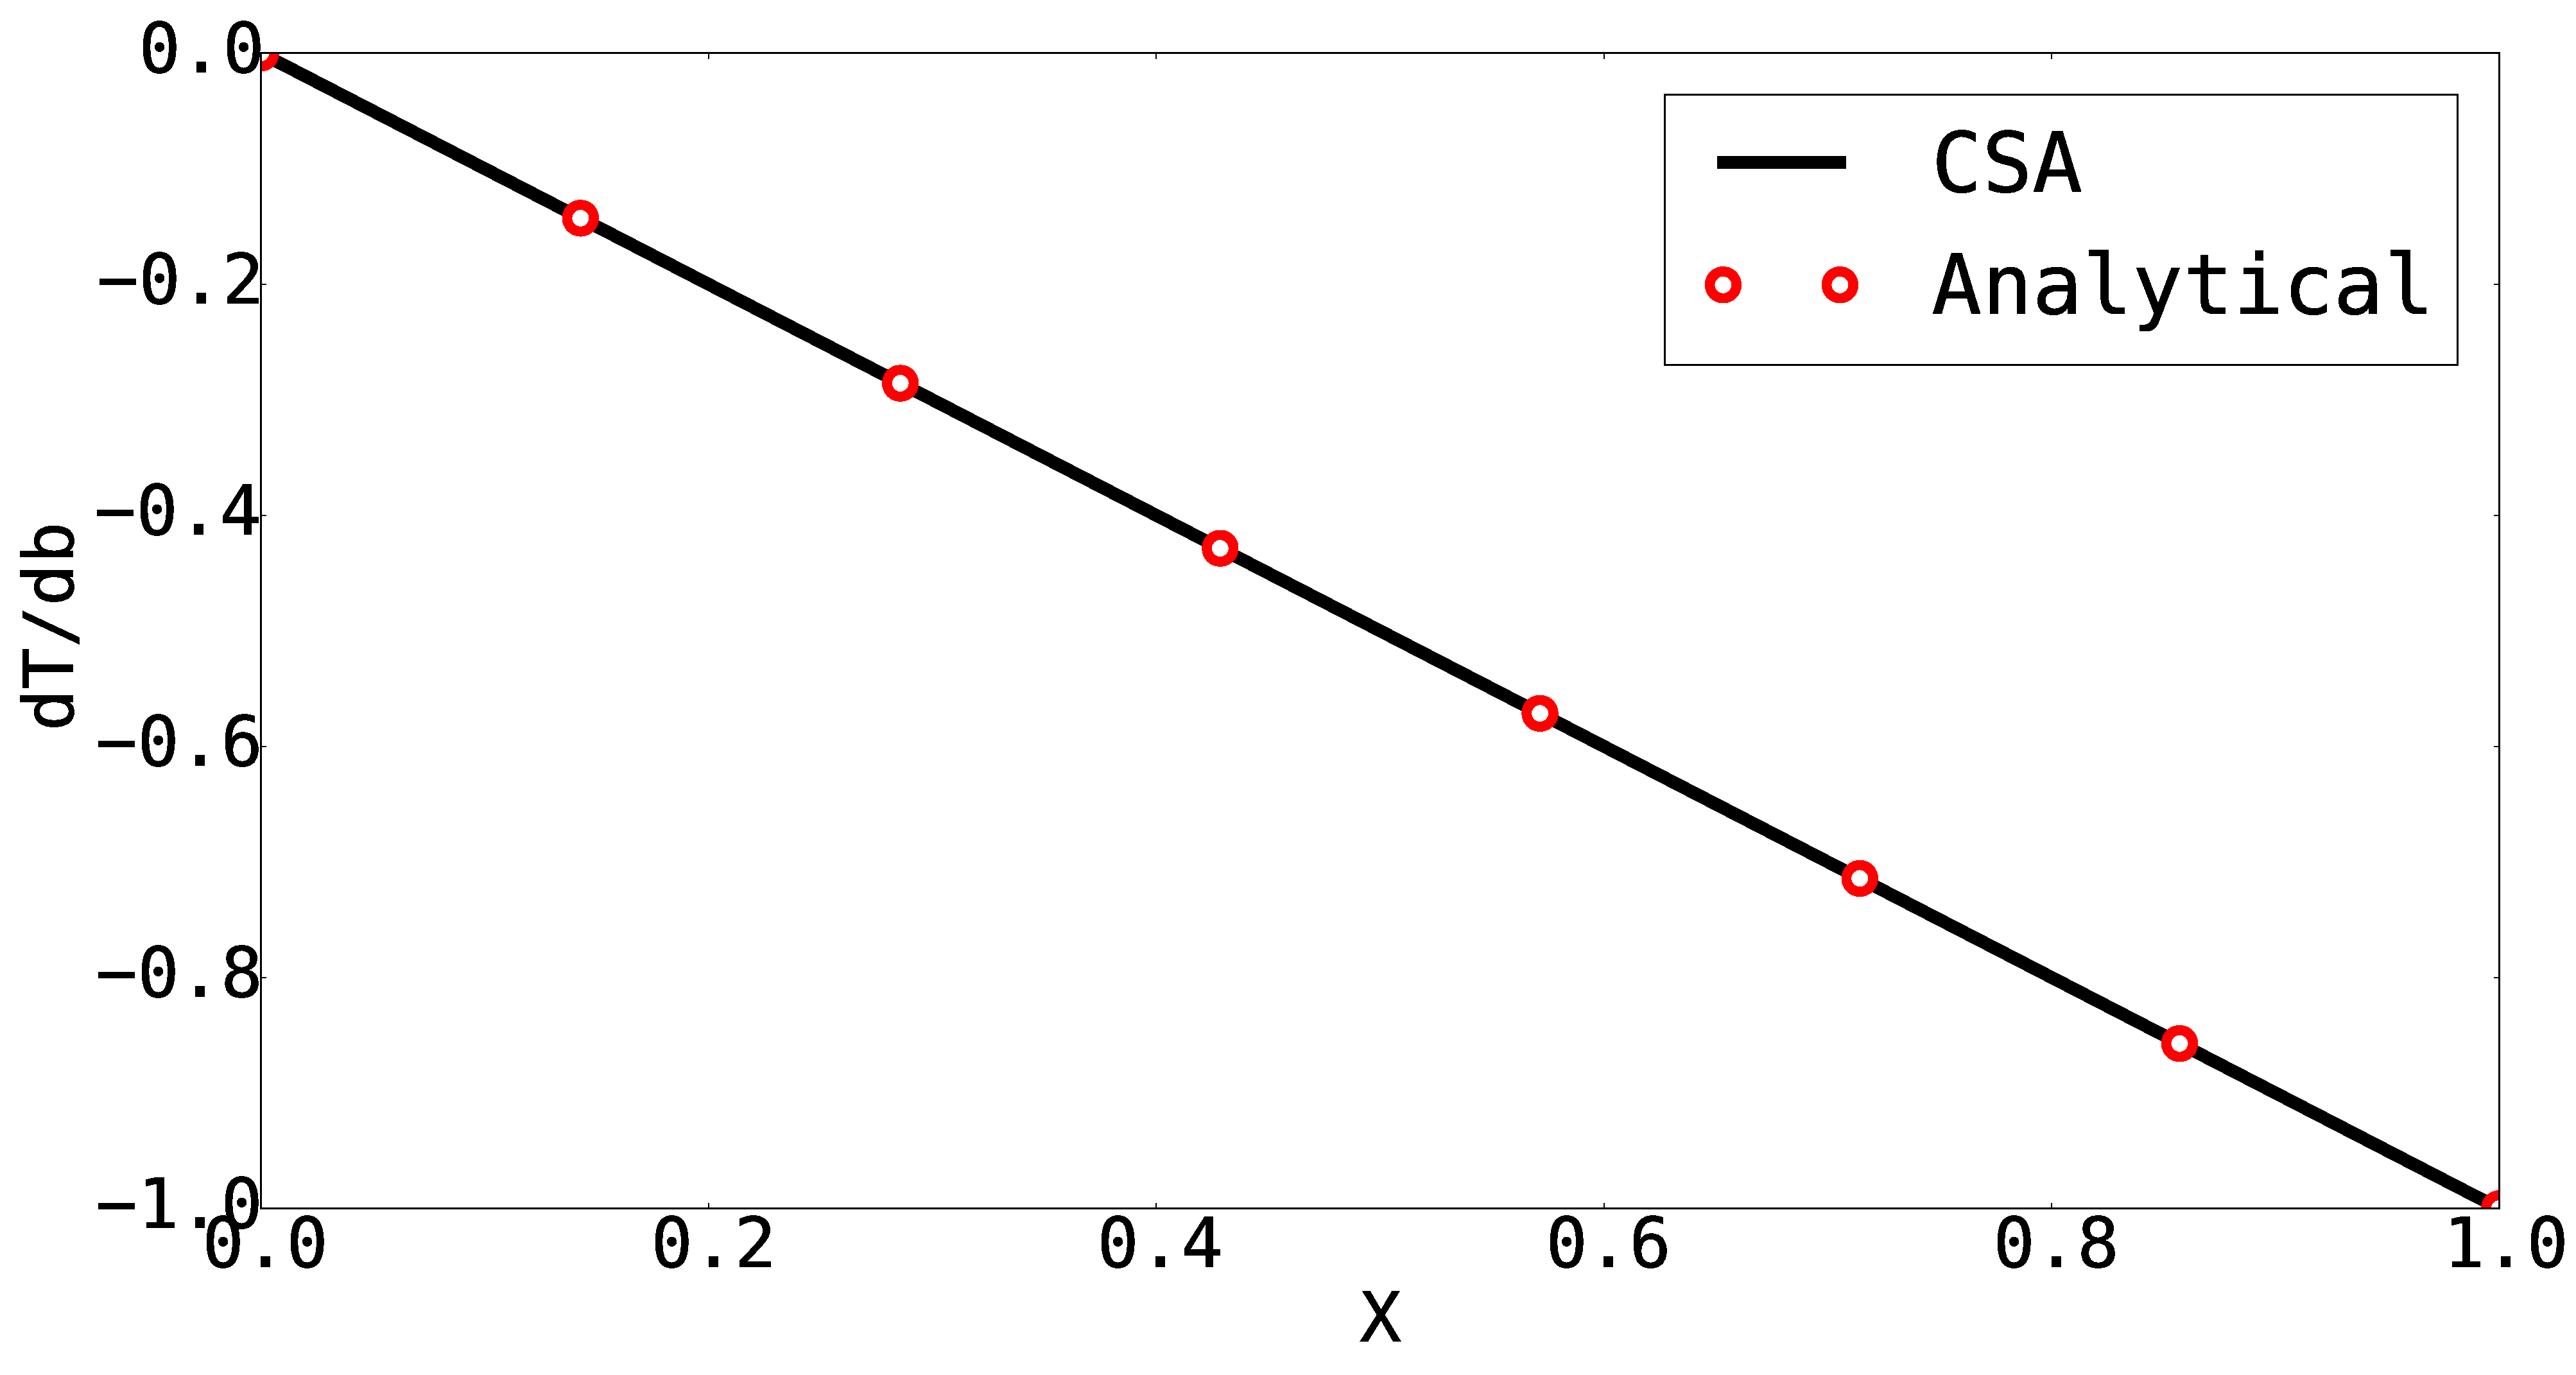
\includegraphics[height=9.00cm]{Chapter_2/figure/SA_CSA_vs_analytical.eps}
	\caption{Comparison between the analytical and continuum sensitivity analysis2 solution for 1D heat equation.}
	\label{fig:C2_verificationOfSolver}
\end{figure}

It should be noted that the sensitivity equations are derived and solved in the local form. This does not include the effect of nodes moving in the computational domain. If the analysis requires the sensitivity at the material points, an additional step is required to convert the local sensitivities to their total form using the chain rule as shown in the following equation.

\begin{equation*}
	\frac{DT}{Db} = \frac{\partial t}{\partial b} + \frac{\partial T}{\partial x} \cdot \frac{\partial x}{\partial b}
\end{equation*}

This will add extra cost to the simulation due to additional step for calculating $\partial x/\partial b$. The reason this step exists is due to movement of computational nodes due to change in shape. Therefore, if the computational nodes can be fixed in this, the $\partial x/\partial b$ term will be equal to zero. We out proposing the achieve this using a non-body conformal technique such as immersed boundary method. This will be explained in the next chapter in more details.

% ======================================================================================
\section{Summary}
In summery, we looked at two main approaches used to calculate the sensitivity response of a system. The discrete method is based on differentiating the discretized governing equations whereas in continuum method the governing equation are differentiated first and then discretized. We applied these techniques to a simple 1D problem of heat transfer and calculated the sensitivity of response to shape design parameter. The sensitivities are calculated in the local form for each of these methods and compared with the analytical results where they show good comparison. We also showed that by using the continuum sensitivity analysis we can reuse the differential operators used in the solution of governing equations. This effectively means that the black-box solver used in the simulation step can be reused with new boundary conditions for solving the sensitivity response. As showed in the example problem, this is not possible when using discrete method. This is mainly due to the fact that the discrete operators will be affected by differentiating with respect to design variables. So more details about the analysis needs to be known when using discrete approach compared to the continuum. Continuum sensitivity approach is used in this document due to its ability to treat the analysis as black-box for solving both the governing equations and the sensitivity response. However, the result of sensitivity analysis is still the local sensitivities which needs to be transformed to the total form using the chain rule. This is not favourable because it is another step on top of an already expensive analysis. We are proposing to use a non-body conformal approach such as immersed boundary method for analysis to remove this step from sensitivity calculation.